\documentclass[11pt]{article}
\usepackage{listings}
\usepackage{tikz}
\usepackage{url}
\usepackage{hyperref}
%\usepackage{algorithm2e}
\usetikzlibrary{arrows,automata,shapes,positioning}
\tikzstyle{block} = [rectangle, draw, fill=blue!20, 
    text width=2.5em, text centered, rounded corners, minimum height=2em]
\tikzstyle{bw} = [rectangle, draw, fill=blue!20, 
    text width=3.5em, text centered, rounded corners, minimum height=2em]

\newcommand{\handout}[5]{
  \noindent
  \begin{center}
  \framebox{
    \vbox{
      \hbox to 5.78in { {\bf ECE459: Programming for Performance } \hfill #2 }
      \vspace{4mm}
      \hbox to 5.78in { {\Large \hfill #5  \hfill} }
      \vspace{2mm}
      \hbox to 5.78in { {\em #3 \hfill #4} }
    }
  }
  \end{center}
  \vspace*{4mm}
}

\lstset{basicstyle=\ttfamily \scriptsize}

\newcommand{\lecture}[4]{\handout{#1}{#2}{#3}{#4}{Lecture #1}}
\topmargin 0pt
\advance \topmargin by -\headheight
\advance \topmargin by -\headsep
\textheight 8.9in
\oddsidemargin 0pt
\evensidemargin \oddsidemargin
\marginparwidth 0.5in
\textwidth 6.5in

\parindent 0in
\parskip 1.5ex
%\renewcommand{\baselinestretch}{1.25}

\begin{document}

\lecture{6 --- January 16, 2015}{Winter 2015}{Patrick Lam}{version 1}

\section*{Assignment 1 Discussion}
We talked about how to do assignment 1. The task is to reassemble a
picture that you fetch over the Internet using curl. You get a C
implementation that uses curl to fetch the code over the network and
uses libpng to read and write PNG files. It populates a buffer based
on the input files and outputs a buffer combining the files'
content.

\paragraph{Main Loop.} The main loop looks like this:
\begin{tabbing}
\=   main loop: until all image fragment fetched,\\
\> ~~~~ \=  retrieve the fragment over the network;\\
\> \>  copy bits into our array;\\
\> Then, write all the bits in one PNG file.
\end{tabbing}

You hand in (0) a fix to a resource leak in my code; (1) a pthread
parallelized implementation; (2) a nonblocking I/O implementation
using the libcurl multi-handle interface; and (3) an Amdahl's Law
etc. discussion.

\paragraph{Retrieving the files.} I discussed the API for retrieving
the file:

\begin{lstlisting}
  curl_easy_setopt(curl, CURLOPT_URL, url);

  // do curl request; check for errors
  res = curl_easy_perform(curl);
\end{lstlisting}

(The server then gives you back an arbitrary image fragment and you
have to loop util you get them all.) However, that wasn't
enough. Before that, I had to tell curl where to put the file---it was
to use the {\tt write\_cb} callback function.

    \begin{lstlisting}
  struct bufdata bd; 
  bd.buf = input_buffer; 
  curl_easy_setopt(curl, CURLOPT_WRITEFUNCTION, write_cb);
  curl_easy_setopt(curl, CURLOPT_WRITEDATA, &bd);
    \end{lstlisting}

{\tt write\_cb} puts data in {\tt input\_buffer} using a straightforward {\tt
  memcpy}-based implementation. It doesn't do anything fancy, but does
make sure that it doesn't overflow the buffer.

\paragraph{Parsing the input .PNG files.} This consisted of a
bunch of {\tt libpng} magic: {\tt libpng} will put the image data
in a {\tt png\_bytep *} array, where each element points to a row of
pixels.

My {\tt read\_png\_file} function allocates the data. I've
chosen the convention that the caller must free the returned value.
These conventions can trip you up and cause memory leaks if they
aren't inconsistently used. 

Afterwards, {\tt paint\_destination} fills in the output array, pasting together
the fragments.

\paragraph{Writing the output .PNG file.} This is simply symmetric
to the read part.

Note: be sure to free everything! (We'll check.)

\subsection*{Using pthreads}
I found this to be quite easy, but I noticed that people found all sorts
of ways to do this which I hadn't anticipated. In any case, I expect that
you will have to do some refactoring. I sort of on purpose made it not
immediately amenable to refactoring.

You need to start some threads. Then, justify why the threads are not
interfering. Time the result.

\subsection*{Nonblocking I/O}
This part is more complicated than using threads. It is typically lower
overhead (why?) and good for servers which handle lots of connections.
But it is also more of a pain to program. On the other hand, you don't have
to worry about shared state.

\paragraph{JavaScript option.} 
As an alternate option, you were allowed to use either {\tt node.js}
or client-side JavaScript to do the nonblocking I/O. You are on your
own for this option. Let me know; I'll mark those solutions myself.

\section*{Asynchronous/non-blocking I/O}

Let's start with some juicy quotes.

\begin{center}
  \fbox{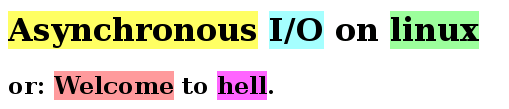
\includegraphics[width=.7\textwidth]{L06/aio-linux.png}}\\
{\scriptsize (mirrored at \url{compgeom.com/~piyush/teach/4531_06/project/hell.html})}
   \\[2em]

   ``Asynchronous I/O, for example, is often infuriating.''\\
\hfill --- Robert Love. {\em Linux System Programming, 2nd ed, } page 215.

\end{center}

To motivate the need for non-blocking I/O, consider some standard I/O code:

\begin{lstlisting}
    fd = open(...);
    read(...);
    close(fd);
\end{lstlisting}

This isn't very performant. The problem is that the {\tt read} call will
{\em block}. So, your program doesn't get to use the zillions of CPU cycles that
are happening while the I/O operation is occurring.

\paragraph{As seen previously: threads.} That can be fine if
you have some other code running to do work---for instance, other threads
do a good job mitigating the I/O latency, perhaps doing I/O themselves.
But maybe you would rather not use threads. Why not?

\begin{itemize}
\item potential race conditions;
\item overhead due to per-thread stacks; or
\item limitations due to maximum numbers of threads.
\end{itemize}

\paragraph{Live coding example.} To illustrate the max-threads
issue, we wrote {\tt threadbomb.c}, which explored how many simultaneous threads
one could start on my computer.

\paragraph{Non-blocking I/O.} The main point of this lecture, though,
is non-blocking/asynchronous I/O. The simplest example:

\begin{lstlisting}
    fd = open(..., O_NONBLOCK);
    read(...); // returns instantly!
    close(fd);
\end{lstlisting}

In principle, the {\tt read} call is supposed to return instantly,
whether or not results are ready. That was easy!

Well, not so much. The {\tt O\_NONBLOCK} flag actually only has the
desired behaviour on sockets. The semantics of {\tt O\_NONBLOCK} is
for I/O calls to not block, in the sense that they should never wait
for data while there is no data available.

Unfortunately, files always have data available. Under Linux, you'd have
to use {\tt aio} calls to be able to send requests to the I/O subsystem
asynchronously and not, for instance, wait for the disk to spin up.
We won't talk about them, but they operate along the same lines as what
we will see. They just have a different API.

\paragraph{Conceptual view: non-blocking I/O.} Fundamentally,
there are two ways to find out whether I/O is ready to be queried:
polling (under UNIX, implemented via {\tt select}, {\tt poll},
and {\tt epoll}) and interrupts (under UNIX, signals).

We will describe {\tt epoll} in lecture. It is the most modern and
flexible interface. Unfortunately, I didn't realize that the obvious
{\tt curl} interface does not work with {\tt epoll} but instead with
{\tt select}.  There is different syntax but the ideas are the same.

The key idea is to give {\tt epoll} a bunch of file descriptors and
wait for events to happen. In particular:
     \begin{itemize}
       \item create an epoll instance ({\tt epoll\_create1});
       \item populate it with file descriptors ({\tt epoll\_ctl}); and
       \item wait for events ({\tt epoll\_wait}).
     \end{itemize}
Let's run through these steps in order.

\paragraph{Creating an {\tt epoll} instance.} Just use the API:
    \begin{lstlisting}
   int epfd = epoll_create1(0);
    \end{lstlisting}

The return value {\tt epfd} is typed like a UNIX file
descriptor---{\tt int}---but doesn't represent any files; instead, use
it as an identifier, to talk to {\tt epoll}.

The parameter ``{\tt 0}'' represents the flags, but the only available flag
is {\tt EPOLL\_CLOEXEC}. Not interesting to you.

\paragraph{Populating the {\tt epoll} instance.} Next, you'll want
{\tt epfd} to do something. The obvious thing is to add some {\tt fd}
to the set of descriptors watched by {\tt epfd}:
    \begin{lstlisting}
   struct epoll_event event;
   int ret;
   event.data.fd = fd;
   event.events = EPOLLIN | EPOLLOUT;
   ret = epoll_ctl(epfd, EPOLL_CTL_ADD, fd, &event);
    \end{lstlisting}

You can also use {\tt epoll\_ctl} to modify and delete descriptors from {\tt epfd}; read the manpage to find out how.

\paragraph{Waiting on an {\tt epoll} instance.} Having completed
the setup, we're ready to wait for events on any file descriptor in {\tt epfd}.
    \begin{lstlisting}
  #define MAX_EVENTS 64

  struct epoll_event events[MAX_EVENTS];
  int nr_events;

  nr_events = epoll_wait(epfd, events, MAX_EVENTS, -1);
    \end{lstlisting}

The given {\tt -1} parameter means to wait potentially forever;
otherwise, the parameter indicates the number of milliseconds to wait.
(It is therefore ``easy'' to sleep for some number of milliseconds by
starting an {\tt epfd} and using {\tt epoll\_wait}; takes two function
calls instead of one, but allows sub-second latency.)

Upon return from {\tt epoll\_wait}, we know that we have {\tt
  nr\_events} events ready.

\subsection*{Level-Triggered and Edge-Triggered Events}
One relevant concept for these polling APIs is the concept of
\emph{level-triggered} versus \emph{edge-triggered}.  The default {\tt
  epoll} behavious is level-triggered: it returns whenever data is
ready. One can also specify (via {\tt epoll\_ctl}) edge-triggered
behaviour: return whenever there is a change in readiness.

We'll have a live coding demo in lecture 7.

\subsection*{Asynchronous I/O}
As mentioned above, the POSIX standard defines {\tt aio} calls.
Unlike just giving the {\tt O\_NONBLOCK} flag, using {\tt aio} works
for disk as well as sockets.

\paragraph{Key idea.} You specify the action to occur when I/O is ready:
    \begin{itemize}
      \item nothing;
      \item start a new thread; or
      \item raise a signal.
    \end{itemize}

Your code submits the requests using e.g. {\tt aio\_read} and {\tt aio\_write}.
If needed, wait for I/O to happen using {\tt aio\_suspend}.

\paragraph{Nonblocking I/O with curl.} The next lecture notes give more clue
about nonblocking I/O with curl. Although it doesn't work with {\tt epoll}
but rather {\tt select}, it uses the same ideas---we'll therefore see two
(three, with aio) different implementations of the same idea. 
Briefly, you:
\begin{itemize}
\item build up a set of descriptors;
\item invoke the transfers and wait for them to finish; and
\item see how things went.
\end{itemize}

\section*{Race Conditions}
We'll next use our knowledge of three address code to analyze
potential race conditions more rigourously.

\paragraph{Definition.} A race occurs when you have two concurrent accesses to the
same memory location, at least one of which is a {\bf write}.

When there's a race, the final state may not be the same as running
one access to completion and then the other. (But it sometimes is.)
Race conditions typically arise between variables which are shared
between threads.

\paragraph{Example.}
\begin{lstlisting}
#include <stdlib.h>
#include <stdio.h>
#include <pthread.h>

void* run1(void* arg)
{
    int* x = (int*) arg;
    *x += 1;
}

void* run2(void* arg)
{
    int* x = (int*) arg;
    *x += 2;
}

int main(int argc, char *argv[])
{
    int* x = malloc(sizeof(int));
    *x = 1;
    pthread_t t1, t2;
    pthread_create(&t1, NULL, &run1, x);
    pthread_join(t1, NULL);
    pthread_create(&t2, NULL, &run2, x);
    pthread_join(t2, NULL);
    printf("%d\n", *x);
    free(x);
    return EXIT_SUCCESS;
}
\end{lstlisting}

\noindent
Question: Do we have a data race? Why or why not?
\vspace*{2em}
%No, we don't. Only one thread is active at a time.

\paragraph{Example 2.} Here's another example; keep the same thread definitions.
\begin{lstlisting}
int main(int argc, char *argv[])
{
    int* x = malloc(sizeof(int));
    *x = 1;
    pthread_t t1, t2;
    pthread_create(&t1, NULL, &run1, x);
    pthread_create(&t2, NULL, &run2, x);
    pthread_join(t1, NULL);
    pthread_join(t2, NULL);
    printf("%d\n", *x);
    free(x);
    return EXIT_SUCCESS;
}
\end{lstlisting}

Now do we have a data race? Why or why not?
\vspace*{2em}

% Yes, we do. We have 2 threads concurrently accessing the same data.

\paragraph{Tracing our Example Data Race.} 
What are the possible outputs? (Assume that initially {\tt *x} is 1.)
We'll look at the three-address code to tell.

\hspace*{.2\textwidth}\begin{minipage}{.8\textwidth}
\begin{lstlisting}[numbers=left]
run1                          run2   
D.1 = *x;                     D.1 = *x;
D.2 = D.1 + 1;                D.2 = D.1 + 2
*x = D.2;                     *x = D.2;
  \end{lstlisting}
\end{minipage}

Memory reads and writes are key in data~races.

Let's call the read and write from {\tt run1} R1 and W1; R2 and W2
from {\tt run2}. Assuming a sane\footnote{sequentially consistent; sadly, many
widely-used models are wilder than this.}
memory model, $R_n$ must precede $W_n$.

\newpage
Here are all possible orderings:
  \begin{center}
    \begin{tabular}{llll|l}
\multicolumn{4}{c|}{Order} & {\tt *x}\\
\hline
R1 & W1 & R2 & W2 & 4 \\
R1 & R2 & W1 & W2 & 3 \\
R1 & R2 & W2 & W1 & 2 \\
R2 & W2 & R1 & W1 & 4 \\
R2 & R1 & W2 & W1 & 2 \\
R2 & R1 & W1 & W2 & 3 \\
    \end{tabular}
  \end{center}

\subsection*{Detecting Data Races Automatically}  
Dynamic and static tools exist. They can help you find data races in
your program. {\tt helgrind} is one such tool. It runs your program 
and analyzes it (and causes a large slowdown).

Run with {\tt valgrind --tool=helgrind <prog>}.

It will warn you of possible data races along with locations. For
useful debugging information, compile your program with debugging
information ({\tt -g} flag for {\tt gcc}).

\paragraph{Helgrind Output for Example.}
\begin{lstlisting}
==5036== Possible data race during read of size 4 at
         0x53F2040 by thread #3
==5036== Locks held: none
==5036==    at 0x400710: run2 (in datarace.c:14)
...
==5036== 
==5036== This conflicts with a previous write of size 4 by
         thread #2
==5036== Locks held: none
==5036==    at 0x400700: run1 (in datarace.c:8)
...
==5036== 
==5036== Address 0x53F2040 is 0 bytes inside a block of size
         4 alloc'd
...
==5036==    by 0x4005AE: main (in datarace.c:19)
\end{lstlisting}



\end{document}
